% Options for packages loaded elsewhere
\PassOptionsToPackage{unicode}{hyperref}
\PassOptionsToPackage{hyphens}{url}
\PassOptionsToPackage{dvipsnames,svgnames,x11names}{xcolor}
\PassOptionsToPackage{space}{xeCJK}
%
\documentclass[
  9pt,
  a4paper,
  ignorenonframetext,
  notheorems]{beamer}
\usepackage{pgfpages}
\setbeamertemplate{caption}[numbered]
\setbeamertemplate{caption label separator}{: }
\setbeamercolor{caption name}{fg=normal text.fg}
\beamertemplatenavigationsymbolshorizontal
% Prevent slide breaks in the middle of a paragraph
\widowpenalties 1 10000
\raggedbottom
\setbeamertemplate{part page}{
  \centering
  \begin{beamercolorbox}[sep=16pt,center]{part title}
    \usebeamerfont{part title}\insertpart\par
  \end{beamercolorbox}
}
\setbeamertemplate{section page}{
  \centering
  \begin{beamercolorbox}[sep=12pt,center]{part title}
    \usebeamerfont{section title}\insertsection\par
  \end{beamercolorbox}
}
\setbeamertemplate{subsection page}{
  \centering
  \begin{beamercolorbox}[sep=8pt,center]{part title}
    \usebeamerfont{subsection title}\insertsubsection\par
  \end{beamercolorbox}
}
\AtBeginPart{
  \frame{\partpage}
}
\AtBeginSection{
  \ifbibliography
  \else
    \frame{\sectionpage}
  \fi
}
\AtBeginSubsection{
  \frame{\subsectionpage}
}

\usepackage{amsmath,amssymb}
\usepackage{iftex}
\ifPDFTeX
  \usepackage[T1]{fontenc}
  \usepackage[utf8]{inputenc}
  \usepackage{textcomp} % provide euro and other symbols
\else % if luatex or xetex
  \usepackage{unicode-math}
  \defaultfontfeatures{Scale=MatchLowercase}
  \defaultfontfeatures[\rmfamily]{Ligatures=TeX,Scale=1}
\fi
\usepackage{lmodern}
\usetheme[outer/progressbar=foot,outer/numbering=fraction,inner/sectionpage=none]{metropolis}
\usecolortheme{seahorse}
\usefonttheme{metropolis}
\usefonttheme{serif} % use mainfont rather than sansfont for slide text
\useoutertheme{metropolis}
\ifPDFTeX\else  
    % xetex/luatex font selection
  \setmainfont[]{HelveticaNeue}
  \setsansfont[]{Fira Mono}
  \setmonofont[Scale=0.75,Color=orange]{Fira Mono}
  \ifXeTeX
    \usepackage{xeCJK}
    \setCJKmainfont[]{NanumGothic}
          \fi
  \ifLuaTeX
    \usepackage[]{luatexja-fontspec}
    \setmainjfont[]{NanumGothic}
  \fi
\fi
% Use upquote if available, for straight quotes in verbatim environments
\IfFileExists{upquote.sty}{\usepackage{upquote}}{}
\IfFileExists{microtype.sty}{% use microtype if available
  \usepackage[]{microtype}
  \UseMicrotypeSet[protrusion]{basicmath} % disable protrusion for tt fonts
}{}
\makeatletter
\@ifundefined{KOMAClassName}{% if non-KOMA class
  \IfFileExists{parskip.sty}{%
    \usepackage{parskip}
  }{% else
    \setlength{\parindent}{0pt}
    \setlength{\parskip}{6pt plus 2pt minus 1pt}}
}{% if KOMA class
  \KOMAoptions{parskip=half}}
\makeatother
\usepackage{xcolor}
\geometry{lmargin=.2in,rmargin=.2in,bmargin=.4in}
\newif\ifbibliography
\setlength{\emergencystretch}{3em} % prevent overfull lines
\setcounter{secnumdepth}{-\maxdimen} % remove section numbering

\usepackage{color}
\usepackage{fancyvrb}
\newcommand{\VerbBar}{|}
\newcommand{\VERB}{\Verb[commandchars=\\\{\}]}
\DefineVerbatimEnvironment{Highlighting}{Verbatim}{commandchars=\\\{\}}
% Add ',fontsize=\small' for more characters per line
\usepackage{framed}
\definecolor{shadecolor}{RGB}{241,243,245}
\newenvironment{Shaded}{\begin{snugshade}}{\end{snugshade}}
\newcommand{\AlertTok}[1]{\textcolor[rgb]{0.68,0.00,0.00}{#1}}
\newcommand{\AnnotationTok}[1]{\textcolor[rgb]{0.37,0.37,0.37}{#1}}
\newcommand{\AttributeTok}[1]{\textcolor[rgb]{0.40,0.45,0.13}{#1}}
\newcommand{\BaseNTok}[1]{\textcolor[rgb]{0.68,0.00,0.00}{#1}}
\newcommand{\BuiltInTok}[1]{\textcolor[rgb]{0.00,0.23,0.31}{#1}}
\newcommand{\CharTok}[1]{\textcolor[rgb]{0.13,0.47,0.30}{#1}}
\newcommand{\CommentTok}[1]{\textcolor[rgb]{0.37,0.37,0.37}{#1}}
\newcommand{\CommentVarTok}[1]{\textcolor[rgb]{0.37,0.37,0.37}{\textit{#1}}}
\newcommand{\ConstantTok}[1]{\textcolor[rgb]{0.56,0.35,0.01}{#1}}
\newcommand{\ControlFlowTok}[1]{\textcolor[rgb]{0.00,0.23,0.31}{#1}}
\newcommand{\DataTypeTok}[1]{\textcolor[rgb]{0.68,0.00,0.00}{#1}}
\newcommand{\DecValTok}[1]{\textcolor[rgb]{0.68,0.00,0.00}{#1}}
\newcommand{\DocumentationTok}[1]{\textcolor[rgb]{0.37,0.37,0.37}{\textit{#1}}}
\newcommand{\ErrorTok}[1]{\textcolor[rgb]{0.68,0.00,0.00}{#1}}
\newcommand{\ExtensionTok}[1]{\textcolor[rgb]{0.00,0.23,0.31}{#1}}
\newcommand{\FloatTok}[1]{\textcolor[rgb]{0.68,0.00,0.00}{#1}}
\newcommand{\FunctionTok}[1]{\textcolor[rgb]{0.28,0.35,0.67}{#1}}
\newcommand{\ImportTok}[1]{\textcolor[rgb]{0.00,0.46,0.62}{#1}}
\newcommand{\InformationTok}[1]{\textcolor[rgb]{0.37,0.37,0.37}{#1}}
\newcommand{\KeywordTok}[1]{\textcolor[rgb]{0.00,0.23,0.31}{#1}}
\newcommand{\NormalTok}[1]{\textcolor[rgb]{0.00,0.23,0.31}{#1}}
\newcommand{\OperatorTok}[1]{\textcolor[rgb]{0.37,0.37,0.37}{#1}}
\newcommand{\OtherTok}[1]{\textcolor[rgb]{0.00,0.23,0.31}{#1}}
\newcommand{\PreprocessorTok}[1]{\textcolor[rgb]{0.68,0.00,0.00}{#1}}
\newcommand{\RegionMarkerTok}[1]{\textcolor[rgb]{0.00,0.23,0.31}{#1}}
\newcommand{\SpecialCharTok}[1]{\textcolor[rgb]{0.37,0.37,0.37}{#1}}
\newcommand{\SpecialStringTok}[1]{\textcolor[rgb]{0.13,0.47,0.30}{#1}}
\newcommand{\StringTok}[1]{\textcolor[rgb]{0.13,0.47,0.30}{#1}}
\newcommand{\VariableTok}[1]{\textcolor[rgb]{0.07,0.07,0.07}{#1}}
\newcommand{\VerbatimStringTok}[1]{\textcolor[rgb]{0.13,0.47,0.30}{#1}}
\newcommand{\WarningTok}[1]{\textcolor[rgb]{0.37,0.37,0.37}{\textit{#1}}}

\providecommand{\tightlist}{%
  \setlength{\itemsep}{0pt}\setlength{\parskip}{0pt}}\usepackage{longtable,booktabs,array}
\usepackage{calc} % for calculating minipage widths
\usepackage{caption}
% Make caption package work with longtable
\makeatletter
\def\fnum@table{\tablename~\thetable}
\makeatother
\usepackage{graphicx}
\makeatletter
\def\maxwidth{\ifdim\Gin@nat@width>\linewidth\linewidth\else\Gin@nat@width\fi}
\def\maxheight{\ifdim\Gin@nat@height>\textheight\textheight\else\Gin@nat@height\fi}
\makeatother
% Scale images if necessary, so that they will not overflow the page
% margins by default, and it is still possible to overwrite the defaults
% using explicit options in \includegraphics[width, height, ...]{}
\setkeys{Gin}{width=\maxwidth,height=\maxheight,keepaspectratio}
% Set default figure placement to htbp
\makeatletter
\def\fps@figure{htbp}
\makeatother

\RequirePackage{fontspec} \RequirePackage{calc} \RequirePackage{microtype} \RequirePackage{etoolbox} \RequirePackage{chngcntr} \RequirePackage{scrextend} \RequirePackage{contour} \RequirePackage[normalem]{ulem} \RequirePackage{underscore} \RequirePackage{hyperref} \titlegraphic{
\includegraphics[width=4cm]{images/hanyang.png}} \definecolor{hyublue}{HTML}{0E4A84} \definecolor{hyulightblue}{HTML}{6e92b5} \definecolor{hyusilver}{HTML}{898C8E} \definecolor{hyulightsilver}{HTML}{6a737b} \setbeamercolor{title}{fg=hyublue} \setbeamercolor{frametitle}{bg=hyusilver!25, fg=hyublue} \setbeamercolor{background canvas}{bg=White} \setbeamercolor{block title}{bg=white, fg=hyublue} \setbeamercolor{block body}{bg=white} \setbeamercolor{block title example}{bg=hyulightblue, fg=white} \setbeamercolor{block body example}{bg=hyulightblue!25} \setbeamercolor{progress bar}{fg=hyulightblue} \setbeamertemplate{blocks}[rounded][shadow=false] \setbeamerfont{title}{size=\fontsize{20}{20}} \setbeamerfont{frametitle}{size=\fontsize{14}{20}} %\setbeamerfont{title}{family=\fontfamily{montserrat}\selectfont} \setlength{\leftmargini}{5pt} % set bullet left margin \setlength{\leftmarginii}{5pt}
\makeatletter
\makeatother
\makeatletter
\makeatother
\makeatletter
\@ifpackageloaded{caption}{}{\usepackage{caption}}
\AtBeginDocument{%
\ifdefined\contentsname
  \renewcommand*\contentsname{Table of contents}
\else
  \newcommand\contentsname{Table of contents}
\fi
\ifdefined\listfigurename
  \renewcommand*\listfigurename{List of Figures}
\else
  \newcommand\listfigurename{List of Figures}
\fi
\ifdefined\listtablename
  \renewcommand*\listtablename{List of Tables}
\else
  \newcommand\listtablename{List of Tables}
\fi
\ifdefined\figurename
  \renewcommand*\figurename{Figure}
\else
  \newcommand\figurename{Figure}
\fi
\ifdefined\tablename
  \renewcommand*\tablename{Table}
\else
  \newcommand\tablename{Table}
\fi
}
\@ifpackageloaded{float}{}{\usepackage{float}}
\floatstyle{ruled}
\@ifundefined{c@chapter}{\newfloat{codelisting}{h}{lop}}{\newfloat{codelisting}{h}{lop}[chapter]}
\floatname{codelisting}{Listing}
\newcommand*\listoflistings{\listof{codelisting}{List of Listings}}
\makeatother
\makeatletter
\@ifpackageloaded{caption}{}{\usepackage{caption}}
\@ifpackageloaded{subcaption}{}{\usepackage{subcaption}}
\makeatother
\makeatletter
\@ifpackageloaded{tcolorbox}{}{\usepackage[skins,breakable]{tcolorbox}}
\makeatother
\makeatletter
\@ifundefined{shadecolor}{\definecolor{shadecolor}{rgb}{.97, .97, .97}}
\makeatother
\makeatletter
\makeatother
\makeatletter
\makeatother
\ifLuaTeX
  \usepackage{selnolig}  % disable illegal ligatures
\fi
\IfFileExists{bookmark.sty}{\usepackage{bookmark}}{\usepackage{hyperref}}
\IfFileExists{xurl.sty}{\usepackage{xurl}}{} % add URL line breaks if available
\urlstyle{same} % disable monospaced font for URLs
\hypersetup{
  pdftitle={Introduction to the R language (1)},
  pdfauthor={Seoncheol Park},
  colorlinks=true,
  linkcolor={hyublue},
  filecolor={hyublue},
  citecolor={hyublue},
  urlcolor={hyublue},
  pdfcreator={LaTeX via pandoc}}

\title{Introduction to the R language (1)}
\author{Seoncheol Park}
\date{}

\begin{document}
\frame{\titlepage}
\ifdefined\Shaded\renewenvironment{Shaded}{\begin{tcolorbox}[breakable, sharp corners, frame hidden, interior hidden, borderline west={3pt}{0pt}{shadecolor}, enhanced, boxrule=0pt]}{\end{tcolorbox}}\fi

\begin{frame}[fragile]{2.1 First steps}
\protect\hypertarget{first-steps}{}
\begin{figure}

{\centering 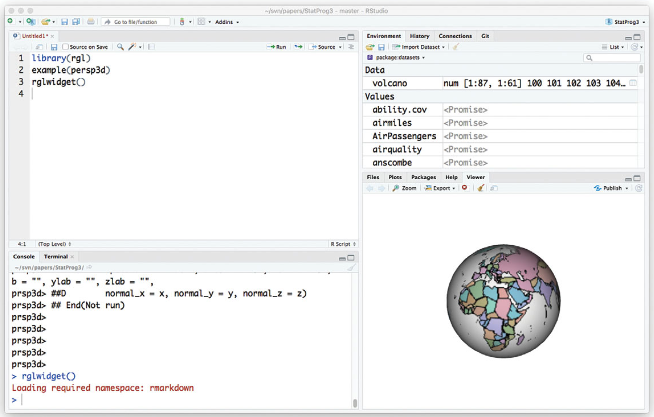
\includegraphics[width=0.7\textwidth,height=\textheight]{images/intro-Rstudiopane.png}

}

\caption{A typical RStudio display}

\end{figure}

\begin{itemize}
\tightlist
\item
  Having opened R or RStudio, you may begin entering and executing
  commands.

  \begin{itemize}
  \tightlist
  \item
    Normally, you will use the \textbf{Source Pane} to type in your
    commands,
  \item
    but you may occasionally use the \textbf{Console Pane} directly. The
    greater-than sign (\texttt{\textgreater{}}) is the prompt symbol
    which appears in the Console Pane.
  \end{itemize}
\end{itemize}
\end{frame}

\begin{frame}[fragile]{2.1.1 R as a calculator}
\protect\hypertarget{r-as-a-calculator}{}
\begin{itemize}
\tightlist
\item
  Anything that can be computed on the calculator app on your smartphone
  can be computed at the R prompt.
\end{itemize}

\begin{block}{Basic operations}
\protect\hypertarget{basic-operations}{}
\begin{itemize}
\tightlist
\item
  The basic operations are

  \begin{itemize}
  \tightlist
  \item
    \texttt{+} (add),
  \item
    \texttt{-} (subtract),
  \item
    \texttt{*} (multiply), and
  \item
    \texttt{/} (divide).
  \end{itemize}
\item
  For example, try
\end{itemize}

\begin{Shaded}
\begin{Highlighting}[]
\DecValTok{5504982}\SpecialCharTok{/}\DecValTok{131071}
\end{Highlighting}
\end{Shaded}

\begin{itemize}
\tightlist
\item
  Upon pressing the Enter key (or \texttt{CTRL-Enter}, or
  \texttt{CMD-Enter}, depending on your system), the result of the above
  division operation, \texttt{42}, appears in the Console Pane, preceded
  by the command you executed, and prefixed by the number 1 in square
  brackets:
\end{itemize}

\begin{Shaded}
\begin{Highlighting}[]
\DecValTok{5504982}\SpecialCharTok{/}\DecValTok{131071}
\end{Highlighting}
\end{Shaded}

\begin{verbatim}
[1] 42
\end{verbatim}

\begin{itemize}
\tightlist
\item
  The \texttt{{[}1{]}} indicates that this is the first (and in this
  case only) result from the command.
\end{itemize}
\end{block}
\end{frame}

\begin{frame}[fragile]
\begin{block}{Multiple commands}
\protect\hypertarget{multiple-commands}{}
\begin{itemize}
\tightlist
\item
  Many commands return multiple values, and each line of results will be
  labeled to aid the user in deciphering the output.
\end{itemize}

\begin{Shaded}
\begin{Highlighting}[]
\CommentTok{\#the sequence of integers from 17 to 58}
\DecValTok{17}\SpecialCharTok{:}\DecValTok{58}
\end{Highlighting}
\end{Shaded}

\begin{verbatim}
 [1] 17 18 19 20 21 22 23 24 25 26 27 28 29 30 31 32 33 34 35 36 37 38 39 40 41
[26] 42 43 44 45 46 47 48 49 50 51 52 53 54 55 56 57 58
\end{verbatim}

The first line starts with the first return value, so is labeled
\texttt{{[}1{]}}; the second line starts with the 23rd, so is labeled
\texttt{{[}23{]}}.
\end{block}

\begin{block}{Parentheses (\texttt{(}, \texttt{)})}
\protect\hypertarget{parentheses}{}
\begin{itemize}
\tightlist
\item
  Everything that you type after a \texttt{\#} sign is assumed to be a
  comment and is ignored by R.
\end{itemize}

\begin{Shaded}
\begin{Highlighting}[]
\DecValTok{5}\SpecialCharTok{:}\NormalTok{(}\DecValTok{2}\SpecialCharTok{*}\DecValTok{3} \SpecialCharTok{+} \DecValTok{10}\NormalTok{) }\CommentTok{\# the result is the same as 5:16}
\end{Highlighting}
\end{Shaded}

\begin{verbatim}
 [1]  5  6  7  8  9 10 11 12 13 14 15 16
\end{verbatim}

\begin{Shaded}
\begin{Highlighting}[]
\NormalTok{(}\DecValTok{7}\SpecialCharTok{:}\DecValTok{10}\NormalTok{) }\SpecialCharTok{+}\NormalTok{ pi }\CommentTok{\# pi is a stored constant}
\end{Highlighting}
\end{Shaded}

\begin{verbatim}
[1] 10.14159 11.14159 12.14159 13.14159
\end{verbatim}
\end{block}
\end{frame}

\begin{frame}[fragile]
\begin{itemize}
\item
  Note that parentheses (\texttt{(}, \texttt{)}) are used to ensure that
  the operations (in this caes, \texttt{:}, \texttt{*}, and \texttt{+})
  are carried out in the order that we desire.
\item
  In the first case, parentheses were necessary to obtain the result we
  wanted to see. The following shows what happens when the parentheses
  are omitted:
\end{itemize}

\begin{Shaded}
\begin{Highlighting}[]
\DecValTok{5}\SpecialCharTok{:}\DecValTok{2}\SpecialCharTok{*}\DecValTok{3} \SpecialCharTok{+} \DecValTok{10}
\end{Highlighting}
\end{Shaded}

\begin{verbatim}
[1] 25 22 19 16
\end{verbatim}

\begin{Shaded}
\begin{Highlighting}[]
\CommentTok{\#comparison:}
\DecValTok{5}\SpecialCharTok{:}\NormalTok{(}\DecValTok{2}\SpecialCharTok{*}\DecValTok{3}\NormalTok{) }\SpecialCharTok{+} \DecValTok{10}
\end{Highlighting}
\end{Shaded}

\begin{verbatim}
[1] 15 16
\end{verbatim}

\begin{itemize}
\tightlist
\item
  The parentheses were not required in \texttt{(7:10)\ +\ pi}. We used
  them anyway, for two reasons.

  \begin{itemize}
  \item
    \begin{enumerate}
    [(1)]
    \tightlist
    \item
      They can help others read and understand the code more quickly.
    \end{enumerate}
  \item
    \begin{enumerate}
    [(1)]
    \setcounter{enumi}{1}
    \tightlist
    \item
      Although R follows strict and consistent rules regarding order of
      operations, we believe it is too easy for a user to forget one or
      more of these rules. Therefore, we recommend using parentheses
      whenever you are unsure.
    \end{enumerate}
  \end{itemize}
\end{itemize}
\end{frame}

\begin{frame}[fragile]
\begin{block}{Other operators}
\protect\hypertarget{other-operators}{}
\begin{itemize}
\tightlist
\item
  R can also be used to compute powers with the \texttt{\^{}} operator.
  For example,
\end{itemize}

\begin{Shaded}
\begin{Highlighting}[]
\DecValTok{3}\SpecialCharTok{\^{}}\DecValTok{4}
\end{Highlighting}
\end{Shaded}

\begin{verbatim}
[1] 81
\end{verbatim}

\begin{itemize}
\tightlist
\item
  Modular arithmetic is also available. For example, you can compute the
  remainder after division of 31 by 7, i.e.~31 (mod 7):
\end{itemize}

\begin{Shaded}
\begin{Highlighting}[]
\DecValTok{31} \SpecialCharTok{\%\%} \DecValTok{7}
\end{Highlighting}
\end{Shaded}

\begin{verbatim}
[1] 3
\end{verbatim}

and the integer part of a fraction as

\begin{Shaded}
\begin{Highlighting}[]
\DecValTok{31} \SpecialCharTok{\%/\%} \DecValTok{7}
\end{Highlighting}
\end{Shaded}

\begin{verbatim}
[1] 4
\end{verbatim}

\begin{itemize}
\tightlist
\item
  We can confirm that 31 is the sum of its remainder plus seven times
  the integer part of the fraction:
\end{itemize}

\begin{Shaded}
\begin{Highlighting}[]
\DecValTok{7}\SpecialCharTok{*}\DecValTok{4} \SpecialCharTok{+} \DecValTok{3}
\end{Highlighting}
\end{Shaded}

\begin{verbatim}
[1] 31
\end{verbatim}
\end{block}
\end{frame}

\begin{frame}[fragile]{2.1.2 Named storage}
\protect\hypertarget{named-storage}{}
\begin{itemize}
\item
  R has a workspace known as the \textbf{global environment} that can be
  used to store the results of calculations, and many other types of
  objects.
\item
  Suppose we would like to store the result of the calculation
  \texttt{1.0025ˆ30} for future use. We will assign this value to an
  object called \texttt{interest.30}. To do this, we type
\end{itemize}

\begin{Shaded}
\begin{Highlighting}[]
\NormalTok{interest}\FloatTok{.30} \OtherTok{\textless{}{-}} \FloatTok{1.0025}\SpecialCharTok{\^{}}\DecValTok{30}
\end{Highlighting}
\end{Shaded}

\begin{itemize}
\item
  We tell R to make the \textbf{assignment} using an arrow that points
  to the left, created with the less-than sign (\texttt{\textless{}})
  and the hyphen (\texttt{-}).
\item
  R also supports using the equals sign (\texttt{=}) in place of the
  arrow in most circumstances. But the authors recommend using the
  arrow, as it makes clear that we are requesting an action (i.e.~an
  assignment), rather than stating a relation (i.e.~that
  \texttt{interest.30} is equal to \texttt{1.0025\^{}30}), or making a
  permanent definition.
\item
  Note that when you run this statement, \textbf{no output appears}: R
  has done what we asked, and is waiting for us to ask for something
  else.
\end{itemize}
\end{frame}

\begin{frame}[fragile]
\begin{itemize}
\tightlist
\item
  You can see the results of this assignment by \textbf{just} typing the
  name of our new object at the prompt:
\end{itemize}

\begin{Shaded}
\begin{Highlighting}[]
\NormalTok{interest}\FloatTok{.30}
\end{Highlighting}
\end{Shaded}

\begin{verbatim}
[1] 1.077783
\end{verbatim}

\begin{itemize}
\tightlist
\item
  We can also use \texttt{interest.30} in further calculations if you
  wish. For example, you can calculate the bank balance after 30 years
  at 0.25\% annual interest, if you start with an initial balance of
  \$3000:
\end{itemize}

\begin{Shaded}
\begin{Highlighting}[]
\NormalTok{initialBalance }\OtherTok{\textless{}{-}} \DecValTok{3000}
\NormalTok{finalBalance }\OtherTok{\textless{}{-}}\NormalTok{ initialBalance }\SpecialCharTok{*}\NormalTok{ interest}\FloatTok{.30}
\NormalTok{finalBalance}
\end{Highlighting}
\end{Shaded}

\begin{verbatim}
[1] 3233.35
\end{verbatim}
\end{frame}

\begin{frame}
\begin{block}{Example 2.1}
\protect\hypertarget{example-2.1}{}
An individual wishes to take out a loan, today, of \(P\) at a monthly
interest rate \(i\). The loan is to be paid back in \(n\) monthly
installments of size \(R\), beginning one month from now.

\textbf{Goal}: calculate \(R\).

Equating the present value \(P\) to the future (discounted) value of the
\(n\) monthly payments \(R\), we have \[
P = R(1+i)^{-1} + R(1+i)^{-2} + \cdots + R(1+i)^{-n}
\] or \[
P = R\sum_{j=1}^n (1+i)^{-j}.
\]

Summing this geometric series and simplifying, we obtain \[
P=R\Big( \frac{1 - (1+i)^{-n}}{i} \Big).
\] This is the formula for the \emph{present value of an annuity}. We
can find \(R\), given \(P\), \(n\) and \(i\) as \[
R= P \frac{i}{1-(1+i)^{-n}}.
\]
\end{block}
\end{frame}

\begin{frame}[fragile]
\begin{itemize}
\tightlist
\item
  In R, we define variables as follows:

  \begin{itemize}
  \tightlist
  \item
    \texttt{principal}: \(P\)
  \item
    \texttt{intRate}: \(i\), and
  \item
    \texttt{n}: \(n\)
  \item
    We will assign the resulting payment value to an object called
    \texttt{payment}.
  \end{itemize}
\end{itemize}

Suppose that the loan amount is \$1500, the interest rate is 1\% and the
number of payments is 10. The resulting code is

\begin{Shaded}
\begin{Highlighting}[]
\NormalTok{intRate }\OtherTok{\textless{}{-}} \FloatTok{0.01}
\NormalTok{n }\OtherTok{\textless{}{-}} \DecValTok{10}
\NormalTok{principal }\OtherTok{\textless{}{-}} \DecValTok{1500}
\NormalTok{payment }\OtherTok{\textless{}{-}}\NormalTok{ principal }\SpecialCharTok{*}\NormalTok{ intRate }\SpecialCharTok{/}\NormalTok{ (}\DecValTok{1} \SpecialCharTok{{-}}\NormalTok{ (}\DecValTok{1} \SpecialCharTok{+}\NormalTok{ intRate)}\SpecialCharTok{\^{}}\NormalTok{(}\SpecialCharTok{{-}}\NormalTok{n))}
\NormalTok{payment}
\end{Highlighting}
\end{Shaded}

\begin{verbatim}
[1] 158.3731
\end{verbatim}
\end{frame}

\begin{frame}[fragile]{2.1.3 Quitting R}
\protect\hypertarget{quitting-r}{}
\begin{itemize}
\tightlist
\item
  To quit your R session, run
\end{itemize}

\begin{Shaded}
\begin{Highlighting}[]
\FunctionTok{q}\NormalTok{()}
\end{Highlighting}
\end{Shaded}

or choose \texttt{Quit\ Seccion...} from the \texttt{File} menu.

\begin{itemize}
\tightlist
\item
  You will then be asked whether to save an image of the current
  workspace, or not, or to cancel.
\end{itemize}

\begin{itemize}
\tightlist
\item
  \textbf{Note}: What happens if your omit the parentheses \texttt{()}
  when attempting to quit:
\end{itemize}

\begin{Shaded}
\begin{Highlighting}[]
\NormalTok{q}
\end{Highlighting}
\end{Shaded}

\begin{verbatim}
function (save = "default", status = 0, runLast = TRUE) 
.Internal(quit(save, status, runLast))
<bytecode: 0x10c1c62e8>
<environment: namespace:base>
\end{verbatim}

\begin{itemize}
\tightlist
\item
  This has happened because \texttt{q} is a \textbf{function} that is
  used to tell R to quit.

  \begin{itemize}
  \tightlist
  \item
    Typing \texttt{q} by itself tells R to show us the contents of the
    function \texttt{q}.
  \item
    By typing \texttt{q()}, we are telling R to call the function
    \texttt{q}. The action of this function is to quit R.
  \end{itemize}
\end{itemize}
\end{frame}

\begin{frame}[fragile]{2.2.1 Functions in R}
\protect\hypertarget{functions-in-r}{}
\begin{itemize}
\tightlist
\item
  Most of the work in R is done through \textbf{functions}.
\end{itemize}

\begin{figure}

{\centering 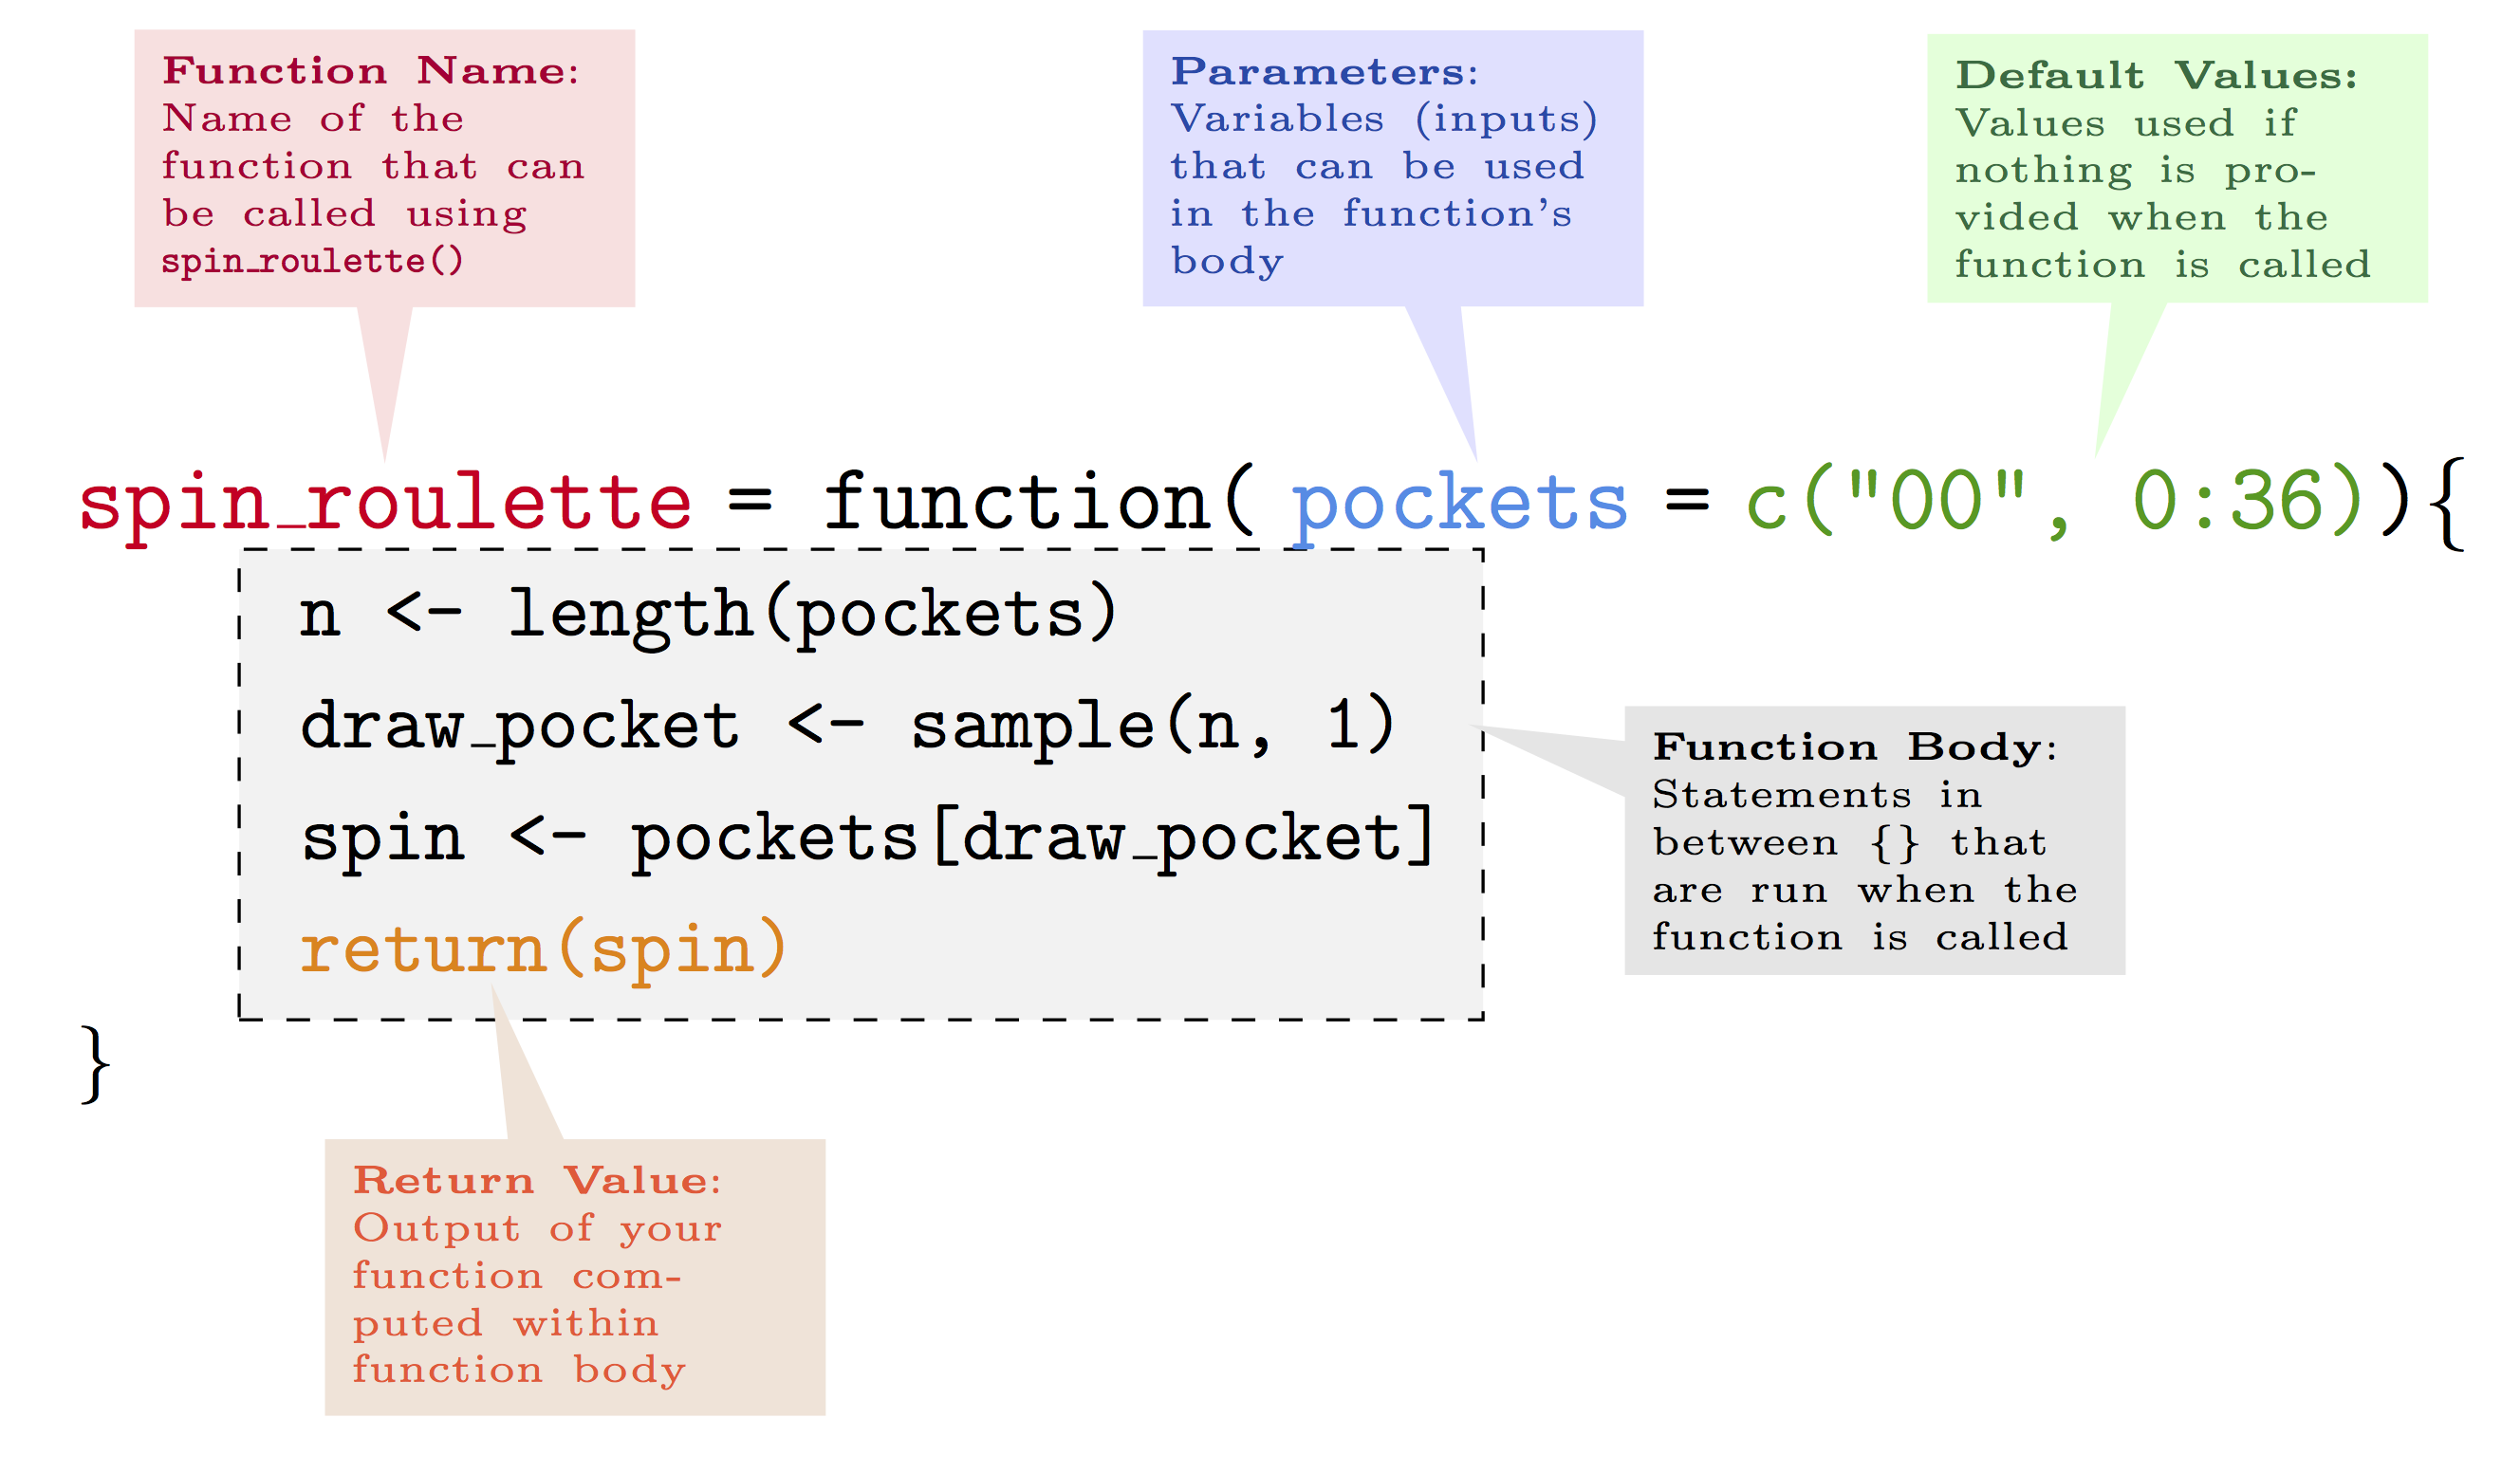
\includegraphics[width=0.7\textwidth,height=\textheight]{images/functionstructure.png}

}

\caption{A typical function structure in R from
https://smac-group.github.io/ds/functions.html.}

\end{figure}

\begin{itemize}
\tightlist
\item
  For example, we saw that to quit R we can type \texttt{q()}. This
  tells R to call the function named \texttt{q}.
\end{itemize}
\end{frame}

\begin{frame}[fragile]
\begin{itemize}
\item
  The parentheses surround the \textbf{argument list}, which in this
  case contains nothing: we just want R to quit, and do not need to tell
  it how.
\item
  We also saw that \texttt{q} is defined as
\end{itemize}

\begin{Shaded}
\begin{Highlighting}[]
\NormalTok{q}
\end{Highlighting}
\end{Shaded}

\begin{verbatim}
function (save = "default", status = 0, runLast = TRUE) 
.Internal(quit(save, status, runLast))
<bytecode: 0x10c1c62e8>
<environment: namespace:base>
\end{verbatim}

\begin{itemize}
\tightlist
\item
  This shows that \texttt{q} is a function that has three arguments:

  \begin{itemize}
  \tightlist
  \item
    \texttt{save},
  \item
    \texttt{status}, and
  \item
    \texttt{runLast}.
  \end{itemize}
\item
  Each of those has a default value:

  \begin{itemize}
  \tightlist
  \item
    \texttt{"default"},
  \item
    \texttt{0}, and
  \item
    \texttt{TRUE}, respectively.
  \end{itemize}
\item
  What happens when we execute \texttt{q()} is that R calls the q
  function with the arguments set to their default values.
\end{itemize}
\end{frame}

\begin{frame}[fragile]
\begin{itemize}
\tightlist
\item
  If we want to change the default values, we specify them when we call
  the function. Arguments are identified in the call (1) by their
  position, or by (2) specifying the name explicitly. Both
\end{itemize}

\begin{Shaded}
\begin{Highlighting}[]
\FunctionTok{q}\NormalTok{(}\StringTok{"no"}\NormalTok{) }
\FunctionTok{q}\NormalTok{(}\AttributeTok{save =} \StringTok{"no"}\NormalTok{)}
\end{Highlighting}
\end{Shaded}

tell R to call \texttt{q} with the first argument set to \texttt{"no"},
i.e.~to quit without saving the workspace. If we had given two arguments
without names, they would apply to \texttt{save} and \texttt{status}.

\begin{itemize}
\tightlist
\item
  If we want to accept the defaults of the early parameters but change
  later ones, we give the name when calling the function, e.g.
\end{itemize}

\begin{Shaded}
\begin{Highlighting}[]
\FunctionTok{q}\NormalTok{(}\AttributeTok{runLast =} \ConstantTok{FALSE}\NormalTok{)}
\end{Highlighting}
\end{Shaded}

or use commas to mark the missing arguments, e.g.

\begin{Shaded}
\begin{Highlighting}[]
\FunctionTok{q}\NormalTok{( , , }\ConstantTok{FALSE}\NormalTok{)}
\end{Highlighting}
\end{Shaded}
\end{frame}

\begin{frame}[fragile]
\begin{itemize}
\tightlist
\item
  Note that we must use \texttt{=} to set arguments.

  \begin{itemize}
  \tightlist
  \item
    If we had written \texttt{q(runLast\ \textless{}-\ FALSE)} it would
    be interpreted quite differently from \texttt{q(runLast\ =\ FALSE)}.
  \item
    The arrow says to put the value \texttt{FALSE} into a variable named
    \texttt{runLast}.
  \item
    We then pass the result of that action (which is the value
    \texttt{FALSE}) as the first argument of \texttt{q()}.
  \item
    Since save is the first argument, it will act like
    \texttt{q(save\ =\ FALSE)}, which is probably not what we wanted.
  \end{itemize}
\end{itemize}
\end{frame}

\begin{frame}[fragile]{2.2.2 R is case-sensitive}
\protect\hypertarget{r-is-case-sensitive}{}
\begin{itemize}
\tightlist
\item
  Consider this:
\end{itemize}

\begin{Shaded}
\begin{Highlighting}[]
\NormalTok{x }\OtherTok{\textless{}{-}} \DecValTok{1}\SpecialCharTok{:}\DecValTok{10}
\FunctionTok{MEAN}\NormalTok{(x)}
\end{Highlighting}
\end{Shaded}

\begin{verbatim}
Error in MEAN(x): could not find function "MEAN"
\end{verbatim}

\begin{itemize}
\tightlist
\item
  Now try
\end{itemize}

\begin{Shaded}
\begin{Highlighting}[]
\NormalTok{MEAN }\OtherTok{\textless{}{-}}\NormalTok{ mean}
\FunctionTok{MEAN}\NormalTok{(x)}
\end{Highlighting}
\end{Shaded}

\begin{verbatim}
[1] 5.5
\end{verbatim}

\begin{itemize}
\tightlist
\item
  The function \texttt{mean()} is built in to R. R considers
  \texttt{MEAN} to be a different function, because it is
  case-sensitive: \texttt{m} is different from \texttt{M}.
\end{itemize}
\end{frame}

\begin{frame}[fragile]{2.2.3 Listing the objects in the workspace}
\protect\hypertarget{listing-the-objects-in-the-workspace}{}
\begin{itemize}
\tightlist
\item
  A list of all objects in the current workspace can be printed to the
  screen using the \texttt{objects()} function:
\end{itemize}

\begin{Shaded}
\begin{Highlighting}[]
\FunctionTok{objects}\NormalTok{()}
\end{Highlighting}
\end{Shaded}

\begin{verbatim}
 [1] "finalBalance"    "has_annotations" "initialBalance"  "interest.30"    
 [5] "intRate"         "MEAN"            "n"               "payment"        
 [9] "principal"       "x"              
\end{verbatim}

\begin{itemize}
\item
  A synonym for \texttt{objects()} is \texttt{ls()}. In RStudio the
  Environment Pane shows both the names and abbreviated displays of the
  objects' values.
\item
  If we quit our R session without saving the workspace image, then
  these objects will disappear.
\item
  If we save the workspace image, then the workspace will be restored at
  our next R session.
\end{itemize}
\end{frame}

\begin{frame}[fragile]{2.3.1 Numeric vectors}
\protect\hypertarget{numeric-vectors}{}
\begin{itemize}
\tightlist
\item
  A numeric vector is a list of numbers. The \texttt{c()} function is
  used to collect things together into a vector.
\end{itemize}

\begin{Shaded}
\begin{Highlighting}[]
\FunctionTok{c}\NormalTok{(}\DecValTok{0}\NormalTok{, }\DecValTok{7}\NormalTok{, }\DecValTok{8}\NormalTok{)}
\end{Highlighting}
\end{Shaded}

\begin{verbatim}
[1] 0 7 8
\end{verbatim}

\begin{itemize}
\tightlist
\item
  Again, we can assign this to a named object:
\end{itemize}

\begin{Shaded}
\begin{Highlighting}[]
\NormalTok{x }\OtherTok{\textless{}{-}} \FunctionTok{c}\NormalTok{(}\DecValTok{0}\NormalTok{, }\DecValTok{7}\NormalTok{, }\DecValTok{8}\NormalTok{) }\CommentTok{\# now x is a 3{-}element vector}
\end{Highlighting}
\end{Shaded}

\begin{itemize}
\tightlist
\item
  To see the contents of \texttt{x}, simply type
\end{itemize}

\begin{Shaded}
\begin{Highlighting}[]
\NormalTok{x}
\end{Highlighting}
\end{Shaded}

\begin{verbatim}
[1] 0 7 8
\end{verbatim}
\end{frame}

\begin{frame}[fragile]
\begin{itemize}
\tightlist
\item
  The \texttt{:} symbol can be used to create \textbf{sequences} of
  increasing (or decreasing) values.
\end{itemize}

\begin{Shaded}
\begin{Highlighting}[]
\NormalTok{numbers5to20 }\OtherTok{\textless{}{-}} \DecValTok{5}\SpecialCharTok{:}\DecValTok{20}
\NormalTok{numbers5to20}
\end{Highlighting}
\end{Shaded}

\begin{verbatim}
 [1]  5  6  7  8  9 10 11 12 13 14 15 16 17 18 19 20
\end{verbatim}

\begin{itemize}
\tightlist
\item
  Vectors can be joined together (i.e.~\emph{concatenated}) with the
  \texttt{c} function.
\end{itemize}

\begin{Shaded}
\begin{Highlighting}[]
\FunctionTok{c}\NormalTok{(numbers5to20, x)}
\end{Highlighting}
\end{Shaded}

\begin{verbatim}
 [1]  5  6  7  8  9 10 11 12 13 14 15 16 17 18 19 20  0  7  8
\end{verbatim}

\begin{itemize}
\tightlist
\item
  Here is another example of the use of the \texttt{c()} function.
\end{itemize}

\begin{Shaded}
\begin{Highlighting}[]
\NormalTok{some.numbers }\OtherTok{\textless{}{-}} \FunctionTok{c}\NormalTok{(}\DecValTok{2}\NormalTok{, }\DecValTok{3}\NormalTok{, }\DecValTok{5}\NormalTok{, }\DecValTok{7}\NormalTok{, }\DecValTok{11}\NormalTok{, }\DecValTok{13}\NormalTok{, }\DecValTok{17}\NormalTok{, }\DecValTok{19}\NormalTok{, }\DecValTok{23}\NormalTok{, }\DecValTok{29}\NormalTok{, }\DecValTok{31}\NormalTok{, }\DecValTok{37}\NormalTok{, }\DecValTok{41}\NormalTok{,}
   \DecValTok{43}\NormalTok{, }\DecValTok{47}\NormalTok{, }\DecValTok{59}\NormalTok{, }\DecValTok{67}\NormalTok{, }\DecValTok{71}\NormalTok{, }\DecValTok{73}\NormalTok{, }\DecValTok{79}\NormalTok{, }\DecValTok{83}\NormalTok{, }\DecValTok{89}\NormalTok{, }\DecValTok{97}\NormalTok{, }\DecValTok{103}\NormalTok{, }\DecValTok{107}\NormalTok{, }\DecValTok{109}\NormalTok{, }\DecValTok{113}\NormalTok{, }\DecValTok{119}\NormalTok{)}
\NormalTok{some.numbers}
\end{Highlighting}
\end{Shaded}

\begin{verbatim}
 [1]   2   3   5   7  11  13  17  19  23  29  31  37  41  43  47  59  67  71  73
[20]  79  83  89  97 103 107 109 113 119
\end{verbatim}
\end{frame}

\begin{frame}[fragile]
\begin{itemize}
\tightlist
\item
  \textbf{Note}: If you type this in the R console (not in the RStudio
  Source Pane), R will prompt you with a \texttt{+} sign for the second
  line of input. That means the code is \textbf{incomplete}:
\end{itemize}

\begin{Shaded}
\begin{Highlighting}[]
\CommentTok{\#try this}
\FunctionTok{c}\NormalTok{(numbers5to20, x}
\end{Highlighting}
\end{Shaded}

\begin{itemize}
\tightlist
\item
  We can append \texttt{numbers5to20} to the end of
  \texttt{some.numbers}, and then append the decreasing sequence from 4
  to 1:
\end{itemize}

\begin{Shaded}
\begin{Highlighting}[]
\NormalTok{a.mess }\OtherTok{\textless{}{-}} \FunctionTok{c}\NormalTok{(some.numbers, numbers5to20, }\DecValTok{4}\SpecialCharTok{:}\DecValTok{1}\NormalTok{) }
\NormalTok{a.mess}
\end{Highlighting}
\end{Shaded}

\begin{verbatim}
 [1]   2   3   5   7  11  13  17  19  23  29  31  37  41  43  47  59  67  71  73
[20]  79  83  89  97 103 107 109 113 119   5   6   7   8   9  10  11  12  13  14
[39]  15  16  17  18  19  20   4   3   2   1
\end{verbatim}
\end{frame}

\begin{frame}[fragile]{2.3.2 Extracting elements from vectors}
\protect\hypertarget{extracting-elements-from-vectors}{}
\textbf{Q}. How can we extract the 22nd element of \texttt{a.mess}?

\begin{itemize}
\tightlist
\item
  A way to display the 22nd element of \texttt{a.mess} is to use square
  brackets to extract just that element:
\end{itemize}

\begin{Shaded}
\begin{Highlighting}[]
\NormalTok{a.mess[}\DecValTok{22}\NormalTok{]}
\end{Highlighting}
\end{Shaded}

\begin{verbatim}
[1] 89
\end{verbatim}

\begin{itemize}
\tightlist
\item
  We can extract more than one element at a time.
\end{itemize}

\begin{Shaded}
\begin{Highlighting}[]
\CommentTok{\#3, 6, 7 elts of \textasciigrave{}a.mess\textasciigrave{}}
\NormalTok{a.mess[}\FunctionTok{c}\NormalTok{(}\DecValTok{3}\NormalTok{, }\DecValTok{6}\NormalTok{, }\DecValTok{7}\NormalTok{)]}
\end{Highlighting}
\end{Shaded}

\begin{verbatim}
[1]  5 13 17
\end{verbatim}

\begin{itemize}
\tightlist
\item
  To get the third through seventh element of \texttt{numbers5to20},
  type
\end{itemize}

\begin{Shaded}
\begin{Highlighting}[]
\NormalTok{numbers5to20[}\DecValTok{3}\SpecialCharTok{:}\DecValTok{7}\NormalTok{]}
\end{Highlighting}
\end{Shaded}

\begin{verbatim}
[1]  7  8  9 10 11
\end{verbatim}
\end{frame}

\begin{frame}[fragile]
\begin{itemize}
\tightlist
\item
  Negative indices can be used to avoid certain elements.
\end{itemize}

\begin{Shaded}
\begin{Highlighting}[]
\CommentTok{\#select all but the second and tenth elts of \textasciigrave{}numbers5to20\textasciigrave{}}
\NormalTok{numbers5to20[}\SpecialCharTok{{-}}\FunctionTok{c}\NormalTok{(}\DecValTok{2}\NormalTok{,}\DecValTok{10}\NormalTok{)]}
\end{Highlighting}
\end{Shaded}

\begin{verbatim}
 [1]  5  7  8  9 10 11 12 13 15 16 17 18 19 20
\end{verbatim}

\begin{itemize}
\tightlist
\item
  The third through eleventh elements of \texttt{numbers5to20} can be
  avoided as follows:
\end{itemize}

\begin{Shaded}
\begin{Highlighting}[]
\NormalTok{numbers5to20[}\SpecialCharTok{{-}}\NormalTok{(}\DecValTok{3}\SpecialCharTok{:}\DecValTok{11}\NormalTok{)]}
\end{Highlighting}
\end{Shaded}

\begin{verbatim}
[1]  5  6 16 17 18 19 20
\end{verbatim}

\begin{itemize}
\tightlist
\item
  Using a zero index returns nothing. This is not something that one
  would usually type, but it may be useful in more complicated
  expressions. For example, recall that \texttt{x} contains the vector
  \texttt{(0,7,8)} so that
\end{itemize}

\begin{Shaded}
\begin{Highlighting}[]
\NormalTok{numbers5to20[x]}
\end{Highlighting}
\end{Shaded}

\begin{verbatim}
[1] 11 12
\end{verbatim}
\end{frame}

\begin{frame}[fragile]
\begin{itemize}
\tightlist
\item
  \textbf{Note 1}: Do \textbf{not} mix positive and negative indices. To
  see what happens, observe
\end{itemize}

\begin{Shaded}
\begin{Highlighting}[]
\NormalTok{x[}\FunctionTok{c}\NormalTok{(}\SpecialCharTok{{-}}\DecValTok{2}\NormalTok{, }\DecValTok{3}\NormalTok{)]}
\end{Highlighting}
\end{Shaded}

\begin{verbatim}
Error in x[c(-2, 3)]: only 0's may be mixed with negative subscripts
\end{verbatim}

\begin{itemize}
\item
  The problem is that it is not clear what is to be extracted: do we
  want the third element of x before or after removing the second one?
\item
  \textbf{Note 2}: Always be careful to make sure that vector indices
  are integers. When fractional values are used, they will be truncated
  towards 0. Thus 0.6 becomes 0, as in
\end{itemize}

\begin{Shaded}
\begin{Highlighting}[]
\NormalTok{x[}\FloatTok{0.6}\NormalTok{]}
\end{Highlighting}
\end{Shaded}

\begin{verbatim}
numeric(0)
\end{verbatim}

\begin{itemize}
\tightlist
\item
  The output \texttt{numeric(0)} indicates a numeric vector of length
  zero.
\end{itemize}
\end{frame}

\begin{frame}[fragile]{2.3.3 Vector arithmetic}
\protect\hypertarget{vector-arithmetic}{}
\begin{itemize}
\tightlist
\item
  Arithmetic can be done on R vectors. For example, we can multiply all
  elements of \texttt{x} by 3:
\end{itemize}

\begin{Shaded}
\begin{Highlighting}[]
\NormalTok{x}\SpecialCharTok{*}\DecValTok{3}
\end{Highlighting}
\end{Shaded}

\begin{verbatim}
[1]  0 21 24
\end{verbatim}

\begin{itemize}
\tightlist
\item
  Note that the computation is performed \textbf{elementwise}. Addition,
  subtraction, and division by a constant have the same kind of effect.
\end{itemize}

\begin{Shaded}
\begin{Highlighting}[]
\NormalTok{y }\OtherTok{\textless{}{-}}\NormalTok{ x }\SpecialCharTok{{-}} \DecValTok{5}
\NormalTok{y}
\end{Highlighting}
\end{Shaded}

\begin{verbatim}
[1] -5  2  3
\end{verbatim}

\begin{itemize}
\tightlist
\item
  For another example, consider taking the 3rd power of the elements of
  \texttt{x}:
\end{itemize}

\begin{Shaded}
\begin{Highlighting}[]
\NormalTok{x}\SpecialCharTok{\^{}}\DecValTok{3}
\end{Highlighting}
\end{Shaded}

\begin{verbatim}
[1]   0 343 512
\end{verbatim}
\end{frame}

\begin{frame}[fragile]
\begin{itemize}
\tightlist
\item
  In general, the binary operators also work element-by-element when
  applied to pairs of vectors. For example, we can compute
  \(y_i^{x_i}\), for \(i=1,2,3,\)
  i.e.~\((y_1^{x_1}, y_2^{x_2}, y_3^{x_3})\), as follows:
\end{itemize}

\begin{Shaded}
\begin{Highlighting}[]
\NormalTok{y}\SpecialCharTok{\^{}}\NormalTok{x}
\end{Highlighting}
\end{Shaded}

\begin{verbatim}
[1]    1  128 6561
\end{verbatim}

\begin{itemize}
\tightlist
\item
  When the vectors are different lengths, the shorter one is extended by
  \textbf{recycling}: values are repeated, starting at the beginning.
  For example, to see the pattern of remainders of the numbers 1 to 10
  modulo 2 and 3,
\end{itemize}

\begin{Shaded}
\begin{Highlighting}[]
\FunctionTok{c}\NormalTok{(}\DecValTok{1}\NormalTok{, }\DecValTok{1}\NormalTok{, }\DecValTok{2}\NormalTok{, }\DecValTok{2}\NormalTok{, }\DecValTok{3}\NormalTok{, }\DecValTok{3}\NormalTok{, }\DecValTok{4}\NormalTok{, }\DecValTok{4}\NormalTok{, }\DecValTok{5}\NormalTok{, }\DecValTok{5}\NormalTok{, }\DecValTok{6}\NormalTok{, }\DecValTok{6}\NormalTok{, }\DecValTok{7}\NormalTok{, }\DecValTok{7}\NormalTok{, }\DecValTok{8}\NormalTok{, }\DecValTok{8}\NormalTok{, }\DecValTok{9}\NormalTok{, }\DecValTok{9}\NormalTok{, }\DecValTok{10}\NormalTok{, }\DecValTok{10}\NormalTok{) }\SpecialCharTok{\%\%} \DecValTok{2}\SpecialCharTok{:}\DecValTok{3}
\end{Highlighting}
\end{Shaded}

\begin{verbatim}
 [1] 1 1 0 2 1 0 0 1 1 2 0 0 1 1 0 2 1 0 0 1
\end{verbatim}

\begin{itemize}
\tightlist
\item
  R will give a warning if the length of the longer vector is not a
  multiple of the length of the smaller one, because that is often a
  symptom of an error.
\end{itemize}

\begin{Shaded}
\begin{Highlighting}[]
\FunctionTok{c}\NormalTok{(}\DecValTok{1}\NormalTok{, }\DecValTok{1}\NormalTok{, }\DecValTok{2}\NormalTok{, }\DecValTok{2}\NormalTok{, }\DecValTok{3}\NormalTok{, }\DecValTok{3}\NormalTok{, }\DecValTok{4}\NormalTok{, }\DecValTok{4}\NormalTok{, }\DecValTok{5}\NormalTok{, }\DecValTok{5}\NormalTok{, }\DecValTok{6}\NormalTok{, }\DecValTok{6}\NormalTok{, }\DecValTok{7}\NormalTok{, }\DecValTok{7}\NormalTok{, }\DecValTok{8}\NormalTok{, }\DecValTok{8}\NormalTok{, }\DecValTok{9}\NormalTok{, }\DecValTok{9}\NormalTok{, }\DecValTok{10}\NormalTok{, }\DecValTok{10}\NormalTok{) }\SpecialCharTok{\%\%} \DecValTok{2}\SpecialCharTok{:}\DecValTok{4}
\end{Highlighting}
\end{Shaded}

\begin{verbatim}
 [1] 1 1 2 0 0 3 0 1 1 1 0 2 1 1 0 0 0 1 0 1
\end{verbatim}

\textbf{Q}. Do you see the error? -\textgreater{} \textbf{No}.
\end{frame}

\begin{frame}[fragile]{2.3.4 Simple patterned vectors}
\protect\hypertarget{simple-patterned-vectors}{}
\begin{itemize}
\tightlist
\item
  Patterned vectors can also be produced using the \texttt{seq()}
  function as well as the \texttt{rep()} function. For example, the
  sequence of odd numbers less than or equal to 21 can be obtained using
\end{itemize}

\begin{Shaded}
\begin{Highlighting}[]
\FunctionTok{seq}\NormalTok{(}\DecValTok{1}\NormalTok{, }\DecValTok{21}\NormalTok{, }\AttributeTok{by =} \DecValTok{2}\NormalTok{)}
\end{Highlighting}
\end{Shaded}

\begin{verbatim}
 [1]  1  3  5  7  9 11 13 15 17 19 21
\end{verbatim}

\begin{itemize}
\tightlist
\item
  Notice the use of \texttt{by\ =\ 2} here. The \texttt{seq()} function
  has several \textbf{optional parameters}, including one named
  \texttt{by}. If \texttt{by} is not specified, the default value of 1
  will be used.
\end{itemize}
\end{frame}

\begin{frame}[fragile]
\begin{itemize}
\tightlist
\item
  Repeated patterns are obtained using \texttt{rep()}. Consider the
  following examples:
\end{itemize}

\begin{Shaded}
\begin{Highlighting}[]
\FunctionTok{rep}\NormalTok{(}\DecValTok{3}\NormalTok{, }\DecValTok{12}\NormalTok{) }\CommentTok{\# repeat the value 3, 12 times}
\end{Highlighting}
\end{Shaded}

\begin{verbatim}
 [1] 3 3 3 3 3 3 3 3 3 3 3 3
\end{verbatim}

\begin{Shaded}
\begin{Highlighting}[]
\FunctionTok{rep}\NormalTok{(}\FunctionTok{seq}\NormalTok{(}\DecValTok{2}\NormalTok{, }\DecValTok{20}\NormalTok{, }\AttributeTok{by =} \DecValTok{2}\NormalTok{), }\DecValTok{2}\NormalTok{) }\CommentTok{\# repeat the pattern 2 4 ... 20, twice}
\end{Highlighting}
\end{Shaded}

\begin{verbatim}
 [1]  2  4  6  8 10 12 14 16 18 20  2  4  6  8 10 12 14 16 18 20
\end{verbatim}

\begin{Shaded}
\begin{Highlighting}[]
\FunctionTok{rep}\NormalTok{(}\FunctionTok{c}\NormalTok{(}\DecValTok{1}\NormalTok{, }\DecValTok{4}\NormalTok{), }\FunctionTok{c}\NormalTok{(}\DecValTok{3}\NormalTok{, }\DecValTok{2}\NormalTok{)) }\CommentTok{\# repeat 1, 3 times and 4, twice}
\end{Highlighting}
\end{Shaded}

\begin{verbatim}
[1] 1 1 1 4 4
\end{verbatim}

\begin{Shaded}
\begin{Highlighting}[]
\FunctionTok{rep}\NormalTok{(}\FunctionTok{c}\NormalTok{(}\DecValTok{1}\NormalTok{, }\DecValTok{4}\NormalTok{), }\AttributeTok{each =} \DecValTok{3}\NormalTok{)  }\CommentTok{\# repeat each value 3 times}
\end{Highlighting}
\end{Shaded}

\begin{verbatim}
[1] 1 1 1 4 4 4
\end{verbatim}

\begin{Shaded}
\begin{Highlighting}[]
\FunctionTok{rep}\NormalTok{(}\DecValTok{1}\SpecialCharTok{:}\DecValTok{10}\NormalTok{, }\FunctionTok{rep}\NormalTok{(}\DecValTok{2}\NormalTok{, }\DecValTok{10}\NormalTok{)) }\CommentTok{\# repeat each value twice}
\end{Highlighting}
\end{Shaded}

\begin{verbatim}
 [1]  1  1  2  2  3  3  4  4  5  5  6  6  7  7  8  8  9  9 10 10
\end{verbatim}
\end{frame}

\begin{frame}[fragile]{2.3.5 Vectors with random patterns}
\protect\hypertarget{vectors-with-random-patterns}{}
\begin{itemize}
\tightlist
\item
  The \texttt{sample()} function allows us to simulate things like the
  results of the repeated tossing of a 6-sided die.
\end{itemize}

\begin{Shaded}
\begin{Highlighting}[]
\FunctionTok{sample}\NormalTok{(}\DecValTok{1}\SpecialCharTok{:}\DecValTok{6}\NormalTok{, }\AttributeTok{size =} \DecValTok{8}\NormalTok{, }\AttributeTok{replace =} \ConstantTok{TRUE}\NormalTok{) }\CommentTok{\# an imaginary die is tossed 8 times}
\end{Highlighting}
\end{Shaded}

\begin{verbatim}
[1] 1 1 1 1 1 3 1 6
\end{verbatim}
\end{frame}

\begin{frame}[fragile]{2.3.6 Character vectors}
\protect\hypertarget{character-vectors}{}
\begin{itemize}
\tightlist
\item
  Scalars and vectors can be made up of strings of characters instead of
  numbers. All elements of a vector must be of the same type. For
  example,
\end{itemize}

\begin{Shaded}
\begin{Highlighting}[]
\NormalTok{colors }\OtherTok{\textless{}{-}} \FunctionTok{c}\NormalTok{(}\StringTok{"red"}\NormalTok{, }\StringTok{"yellow"}\NormalTok{, }\StringTok{"blue"}\NormalTok{)}
\NormalTok{more.colors }\OtherTok{\textless{}{-}} \FunctionTok{c}\NormalTok{(colors, }\StringTok{"green"}\NormalTok{, }\StringTok{"magenta"}\NormalTok{, }\StringTok{"cyan"}\NormalTok{) }\CommentTok{\# this appended some new elements to colors}
\NormalTok{z }\OtherTok{\textless{}{-}} \FunctionTok{c}\NormalTok{(}\StringTok{"red"}\NormalTok{, }\StringTok{"green"}\NormalTok{, }\DecValTok{1}\NormalTok{) }\CommentTok{\# an attempt to mix data types in a vector}
\end{Highlighting}
\end{Shaded}

\begin{itemize}
\tightlist
\item
  To see the contents of \texttt{more.colors} and \texttt{z}, simply
  type
\end{itemize}

\begin{Shaded}
\begin{Highlighting}[]
\NormalTok{more.colors}
\end{Highlighting}
\end{Shaded}

\begin{verbatim}
[1] "red"     "yellow"  "blue"    "green"   "magenta" "cyan"   
\end{verbatim}

\begin{Shaded}
\begin{Highlighting}[]
\NormalTok{z }\CommentTok{\# 1 has been converted to the character "1"}
\end{Highlighting}
\end{Shaded}

\begin{verbatim}
[1] "red"   "green" "1"    
\end{verbatim}

\begin{itemize}
\tightlist
\item
  There are two basic operations you might want to perform on character
  vectors. To take substrings, use \texttt{substr()}. It takes arguments
  \texttt{substr(x,\ start,\ stop)}, where

  \begin{itemize}
  \tightlist
  \item
    \texttt{x} is a vector of character strings, and
  \item
    \texttt{start} and \texttt{stop} say which characters to keep.
  \end{itemize}
\end{itemize}
\end{frame}

\begin{frame}[fragile]
\begin{itemize}
\tightlist
\item
  For example, to print the first two letters of each color use
\end{itemize}

\begin{Shaded}
\begin{Highlighting}[]
\FunctionTok{substr}\NormalTok{(colors, }\DecValTok{1}\NormalTok{, }\DecValTok{2}\NormalTok{)}
\end{Highlighting}
\end{Shaded}

\begin{verbatim}
[1] "re" "ye" "bl"
\end{verbatim}

\begin{itemize}
\tightlist
\item
  The other basic operation is building up strings by concatenation
  within elements. Use the \texttt{paste()} function for this. For
  example,
\end{itemize}

\begin{Shaded}
\begin{Highlighting}[]
\FunctionTok{paste}\NormalTok{(colors, }\StringTok{"flowers"}\NormalTok{)}
\end{Highlighting}
\end{Shaded}

\begin{verbatim}
[1] "red flowers"    "yellow flowers" "blue flowers"  
\end{verbatim}
\end{frame}

\begin{frame}[fragile]
\begin{itemize}
\tightlist
\item
  There are two optional parameters to \texttt{paste()}.

  \begin{itemize}
  \tightlist
  \item
    The \texttt{sep} parameter controls what goes between the components
    being pasted together.
  \item
    The \texttt{paste0()} function is a shorthand way to set
    \texttt{sep\ =\ ""}:
  \item
    The collapse parameter to \texttt{paste()} allows all the components
    of the resulting vector to be collapsed into a single string:
  \end{itemize}
\end{itemize}

\begin{Shaded}
\begin{Highlighting}[]
\FunctionTok{paste}\NormalTok{(}\StringTok{"several "}\NormalTok{, colors, }\StringTok{"s"}\NormalTok{, }\AttributeTok{sep =} \StringTok{""}\NormalTok{)}
\end{Highlighting}
\end{Shaded}

\begin{verbatim}
[1] "several reds"    "several yellows" "several blues"  
\end{verbatim}

\begin{Shaded}
\begin{Highlighting}[]
\FunctionTok{paste0}\NormalTok{(}\StringTok{"several "}\NormalTok{, colors, }\StringTok{"s"}\NormalTok{)}
\end{Highlighting}
\end{Shaded}

\begin{verbatim}
[1] "several reds"    "several yellows" "several blues"  
\end{verbatim}

\begin{Shaded}
\begin{Highlighting}[]
\FunctionTok{paste}\NormalTok{(}\StringTok{"I like"}\NormalTok{, colors, }\AttributeTok{collapse =} \StringTok{", "}\NormalTok{)}
\end{Highlighting}
\end{Shaded}

\begin{verbatim}
[1] "I like red, I like yellow, I like blue"
\end{verbatim}
\end{frame}

\begin{frame}[fragile]{2.3.7 Factors}
\protect\hypertarget{factors}{}
\begin{itemize}
\tightlist
\item
  Factors offer an alternative way to store character data. A factor
  with four elements and having the two levels, \texttt{control} and
  \texttt{treatment} can be created:
\end{itemize}

\begin{Shaded}
\begin{Highlighting}[]
\NormalTok{grp }\OtherTok{\textless{}{-}} \FunctionTok{c}\NormalTok{(}\StringTok{"control"}\NormalTok{, }\StringTok{"treatment"}\NormalTok{, }\StringTok{"control"}\NormalTok{, }\StringTok{"treatment"}\NormalTok{) }
\NormalTok{grp}
\end{Highlighting}
\end{Shaded}

\begin{verbatim}
[1] "control"   "treatment" "control"   "treatment"
\end{verbatim}

\begin{Shaded}
\begin{Highlighting}[]
\NormalTok{grp }\OtherTok{\textless{}{-}} \FunctionTok{factor}\NormalTok{(grp) }
\NormalTok{grp}
\end{Highlighting}
\end{Shaded}

\begin{verbatim}
[1] control   treatment control   treatment
Levels: control treatment
\end{verbatim}

\begin{itemize}
\tightlist
\item
  Factors can be an efficient way of storing character data when there
  are repeats among the vector elements. This is because the levels of a
  factor are internally coded as integers. To see what the codes are for
  our factor, we can type
\end{itemize}

\begin{Shaded}
\begin{Highlighting}[]
\FunctionTok{as.integer}\NormalTok{(grp)}
\end{Highlighting}
\end{Shaded}

\begin{verbatim}
[1] 1 2 1 2
\end{verbatim}
\end{frame}

\begin{frame}[fragile]
\begin{itemize}
\tightlist
\item
  The labels for the levels are only stored once each, rather than being
  repeated. The codes are indices of the vector of levels:
\end{itemize}

\begin{Shaded}
\begin{Highlighting}[]
\FunctionTok{levels}\NormalTok{(grp)}
\end{Highlighting}
\end{Shaded}

\begin{verbatim}
[1] "control"   "treatment"
\end{verbatim}

\begin{Shaded}
\begin{Highlighting}[]
\CommentTok{\#levels(grp)[as.integer(grp)]}
\end{Highlighting}
\end{Shaded}

\begin{itemize}
\tightlist
\item
  The \texttt{levels()} function can be used to change factor labels as
  well. For example, suppose we wish to change the \texttt{"control"}
  label to \texttt{"placebo"}. Since \texttt{"control"} is the first
  level, we change the first element of the \texttt{levels(grp)} vector:
\end{itemize}

\begin{Shaded}
\begin{Highlighting}[]
\FunctionTok{levels}\NormalTok{(grp)[}\DecValTok{1}\NormalTok{] }\OtherTok{\textless{}{-}} \StringTok{"placebo"}
\end{Highlighting}
\end{Shaded}

\begin{itemize}
\tightlist
\item
  An important use for factors is to list all possible values, even if
  some are not present. For example,
\end{itemize}

\begin{Shaded}
\begin{Highlighting}[]
\NormalTok{sex }\OtherTok{\textless{}{-}} \FunctionTok{factor}\NormalTok{(}\FunctionTok{c}\NormalTok{(}\StringTok{"F"}\NormalTok{, }\StringTok{"F"}\NormalTok{), }\AttributeTok{levels =} \FunctionTok{c}\NormalTok{(}\StringTok{"F"}\NormalTok{, }\StringTok{"M"}\NormalTok{)) }
\NormalTok{sex}
\end{Highlighting}
\end{Shaded}

\begin{verbatim}
[1] F F
Levels: F M
\end{verbatim}

shows that there are two possible values for \texttt{sex}, but only one
is present.
\end{frame}

\begin{frame}[fragile]{2.3.8 More on extracting elements from vectors}
\protect\hypertarget{more-on-extracting-elements-from-vectors}{}
\begin{itemize}
\tightlist
\item
  As for numeric vectors, square brackets \texttt{{[}{]}} are used to
  index factor and character vector elements. For example, the factor
  \texttt{grp} has four elements, so we can print out the third element
  by typing
\end{itemize}

\begin{Shaded}
\begin{Highlighting}[]
\NormalTok{grp[}\DecValTok{3}\NormalTok{]}
\end{Highlighting}
\end{Shaded}

\begin{verbatim}
[1] placebo
Levels: placebo treatment
\end{verbatim}

\begin{itemize}
\tightlist
\item
  We can access the second through fifth elements of
  \texttt{more.colors} as follows:
\end{itemize}

\begin{Shaded}
\begin{Highlighting}[]
\NormalTok{more.colors[}\DecValTok{2}\SpecialCharTok{:}\DecValTok{5}\NormalTok{]}
\end{Highlighting}
\end{Shaded}

\begin{verbatim}
[1] "yellow"  "blue"    "green"   "magenta"
\end{verbatim}
\end{frame}

\begin{frame}[fragile]{2.3.9 Matrices and arrays}
\protect\hypertarget{matrices-and-arrays}{}
\begin{itemize}
\tightlist
\item
  To arrange values into a matrix, we use the \texttt{matrix()}
  function:
\end{itemize}

\begin{Shaded}
\begin{Highlighting}[]
\NormalTok{m }\OtherTok{\textless{}{-}} \FunctionTok{matrix}\NormalTok{(}\DecValTok{1}\SpecialCharTok{:}\DecValTok{6}\NormalTok{, }\AttributeTok{nrow =} \DecValTok{2}\NormalTok{, }\AttributeTok{ncol =} \DecValTok{3}\NormalTok{) }
\NormalTok{m}
\end{Highlighting}
\end{Shaded}

\begin{verbatim}
     [,1] [,2] [,3]
[1,]    1    3    5
[2,]    2    4    6
\end{verbatim}

\begin{itemize}
\tightlist
\item
  We can then access elements using two indices. For example, the value
  in the first row, second column is
\end{itemize}

\begin{Shaded}
\begin{Highlighting}[]
\NormalTok{m[}\DecValTok{1}\NormalTok{, }\DecValTok{2}\NormalTok{]}
\end{Highlighting}
\end{Shaded}

\begin{verbatim}
[1] 3
\end{verbatim}

\begin{itemize}
\tightlist
\item
  Somewhat confusingly, R also allows a matrix to be indexed as a
  vector, using just one value:
\end{itemize}

\begin{Shaded}
\begin{Highlighting}[]
\NormalTok{m[}\DecValTok{4}\NormalTok{]}
\end{Highlighting}
\end{Shaded}

\begin{verbatim}
[1] 4
\end{verbatim}
\end{frame}

\begin{frame}[fragile]
\begin{itemize}
\item
  Here elements are selected in the order in which they are stored
  internally: down the first column, then down the second, and so on.
  This is known as \textbf{column-major storage order}.
\item
  Some computer languages use \textbf{row-major storage order}, where
  values are stored in order from left to right across the first row,
  then left to right across the second, and so on.
\item
  Whole rows or columns of matrices may be selected by leaving one index
  blank:
\end{itemize}

\begin{Shaded}
\begin{Highlighting}[]
\NormalTok{m[}\DecValTok{1}\NormalTok{,]}
\end{Highlighting}
\end{Shaded}

\begin{verbatim}
[1] 1 3 5
\end{verbatim}

\begin{Shaded}
\begin{Highlighting}[]
\NormalTok{m[,}\DecValTok{1}\NormalTok{]}
\end{Highlighting}
\end{Shaded}

\begin{verbatim}
[1] 1 2
\end{verbatim}
\end{frame}

\begin{frame}[fragile]
\begin{itemize}
\tightlist
\item
  A more general way to store data is in an \textbf{array}. Arrays have
  multiple indices, and are created using the array function:
\end{itemize}

\begin{Shaded}
\begin{Highlighting}[]
\NormalTok{a }\OtherTok{\textless{}{-}} \FunctionTok{array}\NormalTok{(}\DecValTok{1}\SpecialCharTok{:}\DecValTok{24}\NormalTok{, }\FunctionTok{c}\NormalTok{(}\DecValTok{3}\NormalTok{, }\DecValTok{4}\NormalTok{, }\DecValTok{2}\NormalTok{)) }
\NormalTok{a}
\end{Highlighting}
\end{Shaded}

\begin{verbatim}
, , 1

     [,1] [,2] [,3] [,4]
[1,]    1    4    7   10
[2,]    2    5    8   11
[3,]    3    6    9   12

, , 2

     [,1] [,2] [,3] [,4]
[1,]   13   16   19   22
[2,]   14   17   20   23
[3,]   15   18   21   24
\end{verbatim}

\begin{Shaded}
\begin{Highlighting}[]
\FunctionTok{dim}\NormalTok{(a) }\CommentTok{\#dimensions of a}
\end{Highlighting}
\end{Shaded}

\begin{verbatim}
[1] 3 4 2
\end{verbatim}
\end{frame}

\begin{frame}[fragile]{Floating point numbers}
\protect\hypertarget{floating-point-numbers}{}
\begin{itemize}
\item
  When R creates an integer, R uses the native \textbf{32-bit integer}
  format, which uses (1) 31 bits to store the number and (2) one bit to
  store the sign of the number.
\item
  Within these limitations, the largest positive number R can hold as an
  integer is \(2^31-1=2147483647\).
\end{itemize}

\begin{Shaded}
\begin{Highlighting}[]
\FunctionTok{as.integer}\NormalTok{(}\DecValTok{2}\SpecialCharTok{\^{}}\DecValTok{31} \SpecialCharTok{{-}} \DecValTok{1}\NormalTok{)}
\end{Highlighting}
\end{Shaded}

\begin{verbatim}
[1] 2147483647
\end{verbatim}

\begin{Shaded}
\begin{Highlighting}[]
\FunctionTok{as.integer}\NormalTok{(}\DecValTok{2}\SpecialCharTok{\^{}}\DecValTok{31}\NormalTok{) }\DocumentationTok{\#\#too large number for the integer type}
\end{Highlighting}
\end{Shaded}

\begin{verbatim}
[1] NA
\end{verbatim}

\begin{itemize}
\tightlist
\item
  Of course, R has no trouble with numbers larger than \(2^{31}-1\).
  However, it will not use the internal integer storage format to hold
  these numbers.
\end{itemize}

\begin{Shaded}
\begin{Highlighting}[]
\DecValTok{2}\SpecialCharTok{\^{}}\DecValTok{32}
\end{Highlighting}
\end{Shaded}

\begin{verbatim}
[1] 4294967296
\end{verbatim}

\begin{Shaded}
\begin{Highlighting}[]
\FunctionTok{class}\NormalTok{(}\DecValTok{2}\SpecialCharTok{\^{}}\DecValTok{32}\NormalTok{)}
\end{Highlighting}
\end{Shaded}

\begin{verbatim}
[1] "numeric"
\end{verbatim}
\end{frame}

\begin{frame}[fragile]
\begin{itemize}
\tightlist
\item
  \textbf{Floating point} numbers provide the way to overcome the
  limitations of binary integers.
\end{itemize}

\begin{Shaded}
\begin{Highlighting}[]
\DecValTok{2}\SpecialCharTok{\^{}}\DecValTok{40}
\end{Highlighting}
\end{Shaded}

\begin{verbatim}
[1] 1.099512e+12
\end{verbatim}

\begin{figure}

{\centering 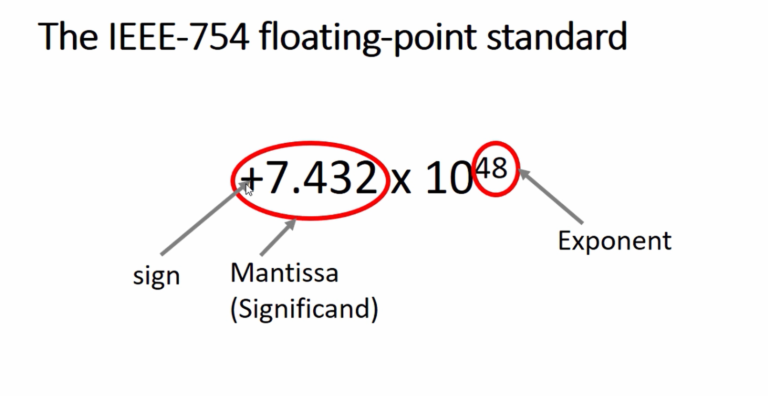
\includegraphics[width=0.7\textwidth,height=\textheight]{images/floating.png}

}

\caption{The IEEE-754 floating-point standard from
https://fastbitlab.com.}

\end{figure}

\begin{itemize}
\tightlist
\item
  For more information about the floating point numbers system, please
  refer
  \href{https://www.geeksforgeeks.org/ieee-standard-754-floating-point-numbers/}{this
  webpage}.
\end{itemize}
\end{frame}

\begin{frame}[fragile]
\begin{itemize}
\item
  As we have seen, floating point can represent a very broad range of
  numbers. However, it cannot also represent every number.
\item
  Machine \(\epsilon\) is defined as the smallest value such that, \[
  1 + \epsilon > 1,
  \] within the floating point system.
\item
  Intuitively, we know that 1 plus any number greater than 0 will be
  greater than 1. But with the number spacing within floating point,
  that is not necessarily the case. Machine \(\epsilon\) is the
  threshold value for representation.
\end{itemize}

\begin{Shaded}
\begin{Highlighting}[]
\NormalTok{.Machine}\SpecialCharTok{$}\NormalTok{double.eps}
\end{Highlighting}
\end{Shaded}

\begin{verbatim}
[1] 2.220446e-16
\end{verbatim}

\begin{Shaded}
\begin{Highlighting}[]
\DecValTok{1} \SpecialCharTok{+}\NormalTok{ .Machine}\SpecialCharTok{$}\NormalTok{double.eps }\SpecialCharTok{\textgreater{}} \DecValTok{1}
\end{Highlighting}
\end{Shaded}

\begin{verbatim}
[1] TRUE
\end{verbatim}

\begin{Shaded}
\begin{Highlighting}[]
\DecValTok{1} \SpecialCharTok{+}\NormalTok{ (.Machine}\SpecialCharTok{$}\NormalTok{double.eps}\SpecialCharTok{/}\DecValTok{2}\NormalTok{) }\SpecialCharTok{\textgreater{}} \DecValTok{1}
\end{Highlighting}
\end{Shaded}

\begin{verbatim}
[1] FALSE
\end{verbatim}
\end{frame}

\begin{frame}[fragile]
\begin{Shaded}
\begin{Highlighting}[]
\FunctionTok{print}\NormalTok{(.Machine}\SpecialCharTok{$}\NormalTok{double.eps, }\AttributeTok{digits=}\DecValTok{20}\NormalTok{)}
\end{Highlighting}
\end{Shaded}

\begin{verbatim}
[1] 2.2204460492503130808e-16
\end{verbatim}

\begin{Shaded}
\begin{Highlighting}[]
\FunctionTok{print}\NormalTok{(.Machine}\SpecialCharTok{$}\NormalTok{double.eps}\SpecialCharTok{/}\DecValTok{2}\NormalTok{, }\AttributeTok{digits=}\DecValTok{20}\NormalTok{)}
\end{Highlighting}
\end{Shaded}

\begin{verbatim}
[1] 1.1102230246251565404e-16
\end{verbatim}

\begin{Shaded}
\begin{Highlighting}[]
\FunctionTok{print}\NormalTok{(}\DecValTok{1} \SpecialCharTok{+}\NormalTok{ .Machine}\SpecialCharTok{$}\NormalTok{double.eps, }\AttributeTok{digits =} \DecValTok{20}\NormalTok{)}
\end{Highlighting}
\end{Shaded}

\begin{verbatim}
[1] 1.000000000000000222
\end{verbatim}

\begin{Shaded}
\begin{Highlighting}[]
\FunctionTok{print}\NormalTok{(}\DecValTok{1} \SpecialCharTok{+}\NormalTok{ .Machine}\SpecialCharTok{$}\NormalTok{double.eps }\SpecialCharTok{/} \DecValTok{2}\NormalTok{, }\AttributeTok{digits =} \DecValTok{20}\NormalTok{)}
\end{Highlighting}
\end{Shaded}

\begin{verbatim}
[1] 1
\end{verbatim}

\begin{itemize}
\tightlist
\item
  R provides a second value to measure the precision of the floating
  point implementation called \texttt{.Machine\$double.neg.eps.}. This
  is the smallest value \(\epsilon\) such that \[
  1 - \epsilon < 1,
  \] within the floating point system.
\end{itemize}

\begin{Shaded}
\begin{Highlighting}[]
\NormalTok{.Machine}\SpecialCharTok{$}\NormalTok{double.neg.eps}
\end{Highlighting}
\end{Shaded}

\begin{verbatim}
[1] 1.110223e-16
\end{verbatim}
\end{frame}

\begin{frame}[fragile]
\begin{itemize}
\tightlist
\item
  The most important effect of this is that certain numbers cannot be
  represented precisely within a floating point system. This is a
  machine-induced error called \textbf{round-off error}.
\end{itemize}

\begin{itemize}
\tightlist
\item
  Round-off error can be brought to prominence with a simple subtraction
  exercise (\textbf{loss of significance}):
\end{itemize}

\begin{Shaded}
\begin{Highlighting}[]
\FloatTok{20.55} \SpecialCharTok{{-}} \FloatTok{19.2} \SpecialCharTok{{-}} \FloatTok{1.35}
\end{Highlighting}
\end{Shaded}

\begin{verbatim}
[1] 1.332268e-15
\end{verbatim}

\begin{Shaded}
\begin{Highlighting}[]
\FloatTok{20.55} \SpecialCharTok{{-}} \FloatTok{1.35} \SpecialCharTok{{-}} \FloatTok{19.2}
\end{Highlighting}
\end{Shaded}

\begin{verbatim}
[1] 0
\end{verbatim}

\begin{Shaded}
\begin{Highlighting}[]
\FunctionTok{print}\NormalTok{(}\FloatTok{20.55} \SpecialCharTok{{-}} \FloatTok{19.2}\NormalTok{, }\AttributeTok{digits=}\DecValTok{20}\NormalTok{)}
\end{Highlighting}
\end{Shaded}

\begin{verbatim}
[1] 1.3500000000000014211
\end{verbatim}

\begin{Shaded}
\begin{Highlighting}[]
\FunctionTok{print}\NormalTok{(}\FloatTok{20.55} \SpecialCharTok{{-}} \FloatTok{1.35}\NormalTok{, }\AttributeTok{digits=}\DecValTok{20}\NormalTok{)}
\end{Highlighting}
\end{Shaded}

\begin{verbatim}
[1] 19.199999999999999289
\end{verbatim}
\end{frame}

\begin{frame}[fragile]{2.4.3 Dates and times}
\protect\hypertarget{dates-and-times}{}
\begin{itemize}
\tightlist
\item
  The standard calendar is very complicated: months of different
  lengths, leap years every four years (with exceptions for whole
  centuries) and so on.
\end{itemize}

\begin{itemize}
\tightlist
\item
  Times are also messy, because there is often an unstated time zone
  (which may change for some dates due to daylight savings time).
\end{itemize}

\begin{itemize}
\tightlist
\item
  There have been several attempts to deal with this in R.

  \begin{itemize}
  \tightlist
  \item
    The base package has the function \texttt{strptime()} to convert
    from strings (e.g.~\texttt{"2020-12-25"}, or \texttt{"12/25/20"}) to
    an internal numerical representation, and \texttt{format()} to
    convert back for printing.
  \item
    Functions in the
    \href{https://github.com/joshuaulrich/xts}{\texttt{xts}} and
    \href{https://lubridate.tidyverse.org}{\texttt{lubridate}} are also
    useful.
  \end{itemize}
\end{itemize}
\end{frame}

\begin{frame}[fragile]{2.4.4 Missing values and other special values}
\protect\hypertarget{missing-values-and-other-special-values}{}
\begin{itemize}
\tightlist
\item
  The missing value symbol is \texttt{NA}. Missing values often arise in
  real data, but they can also arise because of the way calculations are
  performed.
\end{itemize}

\begin{Shaded}
\begin{Highlighting}[]
\NormalTok{some.evens }\OtherTok{\textless{}{-}} \ConstantTok{NULL} \CommentTok{\# creates a vector with no elements }
\NormalTok{some.evens[}\FunctionTok{seq}\NormalTok{(}\DecValTok{2}\NormalTok{, }\DecValTok{20}\NormalTok{, }\DecValTok{2}\NormalTok{)] }\OtherTok{\textless{}{-}} \FunctionTok{seq}\NormalTok{(}\DecValTok{2}\NormalTok{, }\DecValTok{20}\NormalTok{, }\DecValTok{2}\NormalTok{)}
\NormalTok{some.evens}
\end{Highlighting}
\end{Shaded}

\begin{verbatim}
 [1] NA  2 NA  4 NA  6 NA  8 NA 10 NA 12 NA 14 NA 16 NA 18 NA 20
\end{verbatim}

\begin{itemize}
\item
  What happened here is that we assigned values to elements
  \(2,4, \cdots ,20\) but never assigned anything to elements
  \(1, 3, \cdots , 19\), so R uses \texttt{NA} to signal that the value
  is unknown.
\item
  Consider the following:
\end{itemize}

\begin{Shaded}
\begin{Highlighting}[]
\NormalTok{x }\OtherTok{\textless{}{-}} \FunctionTok{c}\NormalTok{(}\DecValTok{0}\NormalTok{, }\DecValTok{1}\NormalTok{, }\DecValTok{2}\NormalTok{)}
\NormalTok{x}\SpecialCharTok{/}\NormalTok{x}
\end{Highlighting}
\end{Shaded}

\begin{verbatim}
[1] NaN   1   1
\end{verbatim}
\end{frame}

\begin{frame}[fragile]
\begin{itemize}
\tightlist
\item
  The \texttt{NaN} symbol denotes a value which is \textbf{not a number}
  which arises as a result of attempting to compute the indeterminate
  0/0. This symbol is sometimes used when a calculation does not make
  sense. In other cases, special values may be shown, or you may get an
  error or warning message.
\end{itemize}

\begin{Shaded}
\begin{Highlighting}[]
\DecValTok{1}\SpecialCharTok{/}\NormalTok{x}
\end{Highlighting}
\end{Shaded}

\begin{verbatim}
[1] Inf 1.0 0.5
\end{verbatim}

Here R has tried to evaluate 1/0 and reports the infinite result as
\texttt{Inf}.

\begin{itemize}
\tightlist
\item
  When there may be missing values, the \texttt{is.na()} function should
  be used to detect them. For instance,
\end{itemize}

\begin{Shaded}
\begin{Highlighting}[]
\FunctionTok{is.na}\NormalTok{(some.evens)}
\end{Highlighting}
\end{Shaded}

\begin{verbatim}
 [1]  TRUE FALSE  TRUE FALSE  TRUE FALSE  TRUE FALSE  TRUE FALSE  TRUE FALSE
[13]  TRUE FALSE  TRUE FALSE  TRUE FALSE  TRUE FALSE
\end{verbatim}
\end{frame}

\begin{frame}[fragile]
The result is a \textbf{logical vector}. The \texttt{!} symbol means
\textbf{not,} so we can locate the non-missing values in
\texttt{some.evens} as follows:

\begin{Shaded}
\begin{Highlighting}[]
\SpecialCharTok{!}\FunctionTok{is.na}\NormalTok{(some.evens)}
\end{Highlighting}
\end{Shaded}

\begin{verbatim}
 [1] FALSE  TRUE FALSE  TRUE FALSE  TRUE FALSE  TRUE FALSE  TRUE FALSE  TRUE
[13] FALSE  TRUE FALSE  TRUE FALSE  TRUE FALSE  TRUE
\end{verbatim}

\begin{itemize}
\tightlist
\item
  We can then display the even numbers only:
\end{itemize}

\begin{Shaded}
\begin{Highlighting}[]
\NormalTok{some.evens[}\SpecialCharTok{!}\FunctionTok{is.na}\NormalTok{(some.evens)]}
\end{Highlighting}
\end{Shaded}

\begin{verbatim}
 [1]  2  4  6  8 10 12 14 16 18 20
\end{verbatim}

Here we have used \texttt{logical\ indexing}.
\end{frame}



\end{document}
